\documentclass{beamer}

\usepackage{array}
\usepackage{dsfont}
\usepackage[normalem]{ulem}

\makeatletter
\def\input@path{{../figures/}}
\makeatother
\graphicspath{{../figures/}}

\newcommand{\tinyspace}{\mspace{1mu}}
\newcommand{\comment}[1]{\textcolor{blue}{%
  \begin{quote}\sf [*** #1 ***]\end{quote}}}

\def\I{\mathds{1}}

\newcommand{\abs}[1]{\lvert #1 \rvert}
\newcommand{\bigabs}[1]{\bigl\lvert #1 \bigr\rvert}
\newcommand{\Bigabs}[1]{\Bigl\lvert #1 \Bigr\rvert}
\newcommand{\biggabs}[1]{\biggl\lvert #1 \biggr\rvert}
\newcommand{\Biggabs}[1]{\Biggl\lvert #1 \Biggr\rvert}

\newcommand{\ip}[2]{\langle #1 , #2\rangle}

\newcommand{\bigip}[2]{\bigl\langle #1, #2 \bigr\rangle}
\newcommand{\Bigip}[2]{\Bigl\langle #1, #2 \Bigr\rangle}
\newcommand{\biggip}[2]{\biggl\langle #1, #2 \biggr\rangle}
\newcommand{\Biggip}[2]{\Biggl\langle #1, #2 \Biggr\rangle}

\newcommand{\norm}[1]{\lVert\tinyspace #1 \tinyspace\rVert}
\newcommand{\bignorm}[1]{\bigl\lVert\tinyspace #1 \tinyspace\bigr\rVert}
\newcommand{\Bignorm}[1]{\Bigl\lVert\tinyspace #1 \tinyspace\Bigr\rVert}
\newcommand{\biggnorm}[1]{\biggl\lVert\tinyspace #1 \tinyspace\biggr\rVert}
\newcommand{\Biggnorm}[1]{\Biggl\lVert\tinyspace #1 \tinyspace\Biggr\rVert}

\newcommand{\tr}{\operatorname{Tr}}
\newcommand{\class}[1]{\mathsf{#1}}

\renewcommand{\thefootnote}{\footnotesize{$\mathparagraph$}} 

\def\X{\mathcal{X}}
\def\Y{\mathcal{Y}}
\def\E{\mathcal{E}}
\def\K{\mathcal{K}}
\def\W{\mathcal{W}}
\def\C{\mathcal{C}}
\def\A{\mathcal{A}}
\def\B{\mathcal{B}}
\def\H{\mathcal{H}}
\def\R{\mathcal{R}}
\def\S{\mathcal{S}}
\def\complex{\mathbb{C}}

\def\BB84{\mathsf{BB84}}
\def\CHSH{\mathsf{CHSH}}

\def \GammaA{\Gamma_{\reg{A}}}
\def \GammaB{\Gamma_{\reg{B}}}
\def \SigmaA{\Sigma_{\reg{A}}}
\def \SigmaB{\Sigma_{\reg{B}}}

\def\ns{\textnormal{ns}}

\newcommand{\setft}[1]{\mathrm{#1}}
\newcommand{\Density}{\setft{D}}
\newcommand{\Pos}{\setft{Pos}}
\newcommand{\Proj}{\setft{Proj}}
\newcommand{\Unitary}{\setft{U}}
\newcommand{\Herm}{\setft{Herm}}
\newcommand{\Lin}{\setft{L}}
\newcommand{\Sep}{\setft{Sep}}
\newcommand{\LOCC}{\setft{LOCC}}
\newcommand{\Ent}{\setft{Ent}}

\def \im{\textnormal{im}}

\newcommand{\microspace}{\mspace{0.5mu}}
\newcommand{\ket}[1]{
  \lvert\microspace #1 \microspace \rangle}
\newcommand{\bra}[1]{
  \langle\microspace #1 \microspace \rvert}

\def\eps{\varepsilon}
\newcommand{\mh}{\textnormal{-}}

\newcommand{\reg}[1]{\mathsf{#1}}

\usepackage{colortbl}
\definecolor{Gray}{gray}{0.90}

\newtheorem{prop}[theorem]{Proposition}

\AtBeginSection[]{
  \begin{frame}
  \vfill
  \centering
  \begin{beamercolorbox}[sep=8pt,center,shadow=true,rounded=true]{title}
    \usebeamerfont{title}\insertsectionhead\par%
  \end{beamercolorbox}
  \vfill
  \end{frame}
}

% ABSTRACT
%Two-player one-round games have served to be an instrumental model in theoretical computer science. Likewise, nonlocal games consider this model when the players have access to an entangled quantum state. In this talk I will consider a broader class of nonlocal games, (extended-nonlocal games), where the referee shares an entangled state along with the players. We will pay particular attention to a type of extended nonlocal game called monogamy-of-entanglement games. Throughout the talk, there will be code examples to help us understand and appreciate these games. The code will make use of MATLAB, and a particularly nice package called QETLAB, which is a library primarily written by Nathaniel Johnston for studying quantum information. 

\title{Monogamy-of-entanglement games}
\subtitle{Theory Seminar}
\author[V. Russo]{Vincent Russo}
\institute[UWaterloo]{University of Waterloo}
\date{August 11, 2016}
\titlegraphic{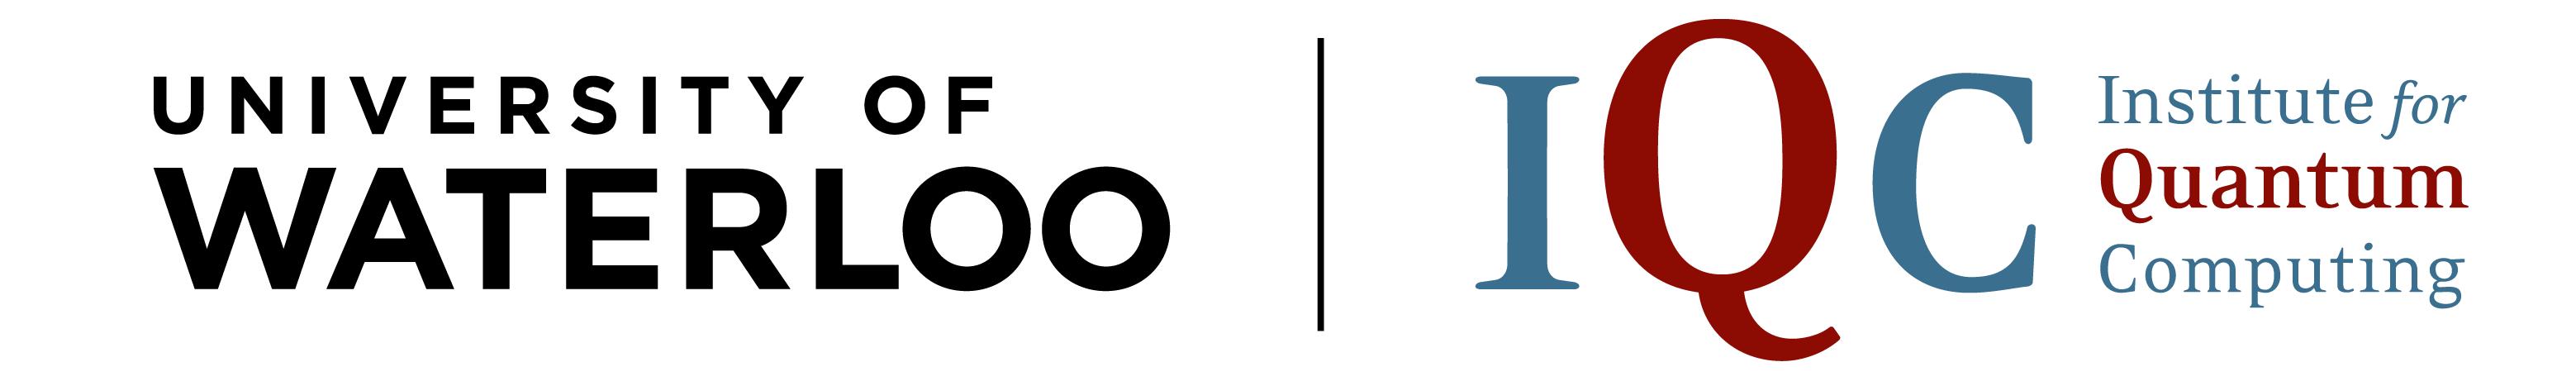
\includegraphics[scale=0.5]{UW_IQC}}

\begin{document}
  {%
    \setbeamertemplate{headline}{}
    \frame{\titlepage}
  }

  \beamertemplatenavigationsymbolsempty
  \addtobeamertemplate{navigation symbols}{}{%
    \usebeamerfont{footline}%
    \usebeamercolor[fg]{footline}%
    \hspace{1em}%
    \insertframenumber/\inserttotalframenumber
  }
  \setbeamercolor{footline}{fg=black}
  % \setbeamerfont{footline}{series=\bfseries}

  \begin{frame}
    \frametitle{Outline}
    \tableofcontents%[part=1,pausesections]
  \end{frame}

%%%%%%%%%%%%%%%%%%%%%%%%%%%%%%%%%%%%%%%%%%%%%%%%%%%%%
  \section{Nonlocal games}
%%%%%%%%%%%%%%%%%%%%%%%%%%%%%%%%%%%%%%%%%%%%%%%%%%%%%

% Nonlocal games:
\begin{frame}
	\frametitle{Nonlocal games}
	A \emph{nonlocal game} is a cooperative game played between \emph{Alice} and \emph{Bob} against a \emph{referee}. 
	\begin{figure}[!htpb] \label{fig:nonlocal-game}
	\begin{center}
		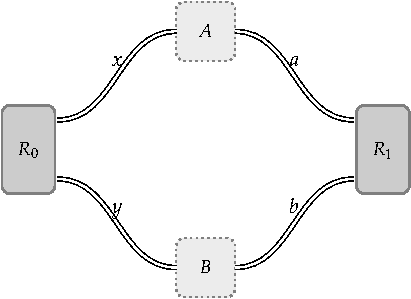
\includegraphics[scale=0.8]{figures/two_player_game.pdf}
	\end{center}
\end{figure}
	\begin{enumerate}
		\item Question and answer sets: $(\SigmaA, \SigmaB)$ and $(\GammaA, \GammaB)$,
		\item Distributions on question pairs: $\pi: \SigmaA \times \SigmaB \rightarrow [0,1]$ ,
		\item A predicate $V : \GammaA \times \GammaB \times \SigmaA \times \SigmaB \rightarrow \{0,1\}$, where 
\[
 V(a,b|x,y) =
  \begin{cases} 
      \hfill 1 \hfill & \text{ if Alice and Bob \textcolor{green}{win}}, \\
      \hfill 0 \hfill & \text{ if Alice and Bob \textcolor{red}{lose}}. \\
  \end{cases}
\]			
	\end{enumerate}
\end{frame}

\begin{frame}
	\frametitle{Strategies and values for nonlocal games}
	Alice and Bob could use different types of \emph{strategies}:
	\vspace{2mm}
	\begin{itemize}
		\item \emph{Classical strategies:} Alice and Bob answer deterministically, determined by functions of $f : \SigmaA \rightarrow \GammaA$ and $g : \SigmaB \rightarrow \GammaB$. 
		\vspace{5mm}
		\item \emph{Quantum strategies:} Alice and Bob share a joint quantum system $\rho \in \Density(\A \otimes \B)$ and allow their answers to be outcomes of measurements on this shared system.		
	\end{itemize}
	\pause 
	\vspace{5mm}
	The \emph{value} of a nonlocal game is the maximal winning probability for the players to win over all strategies of a specified type. 
	\vspace{2mm}
	
For a nonlocal game, $G$, we denote the classical and quantum values as 
	\begin{itemize}
		\item Classical value: $\omega(G)$,
		\item Quantum value: $\omega^*(G)$.
	\end{itemize}
\end{frame}

% Example: CHSH:
\begin{frame}
	\frametitle{Example: The CHSH game}		
	The CHSH game ($G_{\CHSH}$). Question and answer sets over $\{0,1\}$. Question pairs $\{ 00, 01, 10, 11 \}$ selected with equal probability. Winning condition iff $a \oplus b = x \land y$.
	\begin{center}
			$\omega(G_{\CHSH}) < \omega^*(G_{\CHSH})$
	\end{center}

	\begin{itemize}
		\item $\omega(G_{\CHSH}) = \frac{3}{4} = 0.75$:
		\begin{center}
			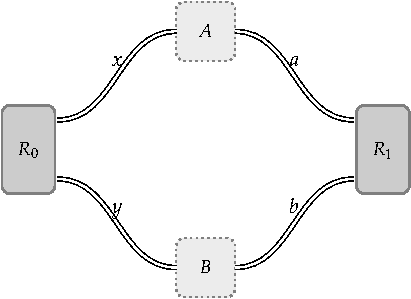
\includegraphics[scale=0.4]{figures/two_player_game.pdf}
		\end{center}
		\item $\omega^*(G_{\CHSH}) = \cos^2(\frac{\pi}{8}) \approx 0.8536$:
		\begin{center}
			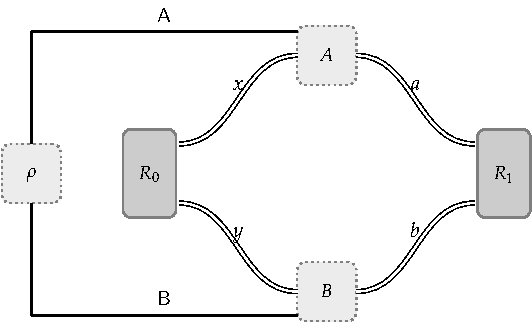
\includegraphics[scale=0.4]{figures/nonlocal_game_2.pdf}
		\end{center}		
	\end{itemize}
\end{frame}

\begin{frame} [noframenumbering]
  \vfill
  \centering
  \begin{beamercolorbox}[sep=8pt,center,shadow=true,rounded=true]{title}
    \usebeamerfont{title}Demo Time: CHSH game in QETLAB \\ \textsc{chsh\_game.m}
  \end{beamercolorbox}
  \vfill
\end{frame}
    

%%%%%%%%%%%%%%%%%%%%%%%%%%%%%%%%%%%%%%%%%%%%%%%%%%%%%
  \section{Extended nonlocal games}
%%%%%%%%%%%%%%%%%%%%%%%%%%%%%%%%%%%%%%%%%%%%%%%%%%%%%    

% Extended nonlocal games:
\begin{frame}
	\frametitle{Extended nonlocal games}
	An \emph{extended nonlocal game} is a nonlocal game where the \emph{referee also holds a quantum system} that he measures provided by Alice and Bob. 
	\begin{figure}[!htpb] \label{fig:extended-nonlocal-game}
	\begin{center}
		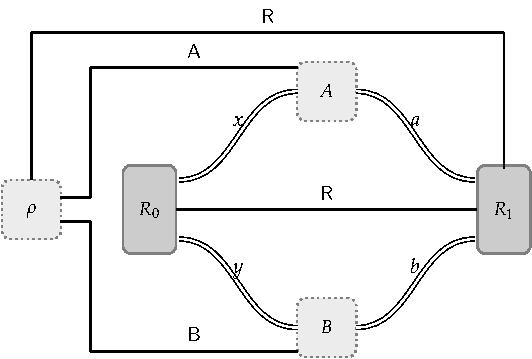
\includegraphics[scale=0.7]{figures/enlg_2.pdf}
	\end{center}
\end{figure}
	\begin{enumerate}
		\item Question and answer sets $(\SigmaA,\SigmaB)$ and $(\GammaA,\GammaB)$. \vspace{1mm}		
		\item Distribution on question pairs: $\pi: \SigmaA \times \SigmaB \rightarrow [0,1]$.\vspace{1mm}
		\item A measurement operator $V: \GammaA \times \GammaB \times \SigmaA \times \SigmaB \rightarrow \Pos(\R)$.
	\end{enumerate}
\end{frame}

\begin{frame}
	\frametitle{Extended nonlocal games: Winning and losing probabilities}
	At the end of the protocol, the referee has: 
		\begin{enumerate}
			\item The state at the end of the protocol: 
				\begin{align*}
					\rho_{a,b}^{x,y} \in \Density(\R).
				\end{align*}
			\item A measurement the referee makes on its part of the state $\rho$: 
			\begin{align*}
				V(a,b|x,y) \in \Pos(\R).
			\end{align*}				
		\end{enumerate}
	The respective winning and losing probabilities are given by
		\begin{align*}
			\biggip{V(a,b|x,y)}{\rho_{a,b}^{x,y}} \quad \textnormal{and} \quad \biggip{\I - V(a,b|x,y)}{\rho_{a,b}^{x,y}}. 
		\end{align*}

\end{frame}

%%%%%%%%%%%%%%%%%%%%%%%%%%%%%%%%%%%%%%%%%%%%%%%%%%%%%
  \section{Monogamy-of-entanglement games}
%%%%%%%%%%%%%%%%%%%%%%%%%%%%%%%%%%%%%%%%%%%%%%%%%%%%%

\begin{frame}
	\frametitle{Monogamy-of-entanglement games}
	Monogamy-of-entanglement games\footnote{[Tomamichel, Fehr, Kaniewski, Wehner, (2013)]}, are a special type of extended nonlocal game. 
\begin{figure}[!htpb] \label{fig:monogamy-of-entanglement game}
	\begin{center}
		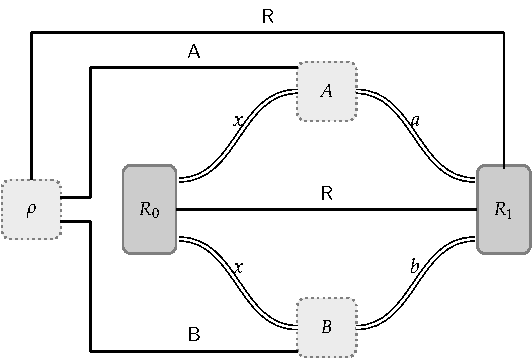
\includegraphics[scale=0.7]{figures/moe_2.pdf}
	\end{center}
\end{figure}
	\begin{enumerate}
		\item Same question and answer sets: $\Sigma = \SigmaA = \SigmaB$ and $\Gamma = \GammaA = \GammaB$. 
		\item Alice and Bob get the same question: $\pi(x,y) = 0$ for $x \not= y$. 
		\item Referee's measurement operator: $R : \Sigma \times \Gamma \rightarrow \Pos(\R)$. 
		\item Winning condition: Iff Alice's output, Bob's output, and the referee's output are all the \emph{equal}. 
	\end{enumerate}
\end{frame}

% Set of density matrices is convex;
% Extreme points of that set are pure states;
% Any density matrix can be written as a convex combination of pure states
% The maximum is therefore achieved by a pure state. 
\begin{frame}
	\frametitle{Standard quantum strategies for monogamy-of-entanglement games}
	A \emph{standard quantum strategy} consists of a tripartite state $\rho \in \Density(\R \otimes \A \otimes \B)$ and sets of local measurements for Alice and Bob. 
	\begin{itemize}
		\item The winning probability for a monogamy-of-entanglement game using a standard quantum strategy is:
			\begin{align*}
				\sum_{x \in \Sigma} \pi(x) \sum_{a \in \Gamma} \biggip{R(a|x) \otimes A_a^x \otimes B_a^x}{\rho}.
			\end{align*}
%		\item Since $\rho$ just needs to be a valid density matrix, we use convexity to assume that $\rho$ is pure (rank-one):
%			\begin{align*}
%				\omega^*(G) = \biggnorm{ \sum_{x \in \Sigma} \pi(x) \sum_{a \in \Gamma} R(a|x) \otimes A_a^x \otimes B_a^x }
%			\end{align*}
	\end{itemize}
The standard quantum value of a monogamy-of-entanglement game, $G$, denoted as $\omega^*(G)$, is the maximal winning probability for Alice and Bob over all standard quantum strategies. 	
\end{frame}

\begin{frame}
	\frametitle{Unentangled strategies for monogamy-of-entanglement games}
	In an \emph{unentangled strategy}, the state $\rho$ prepared by Alice and Bob is fully separable, that is
	\begin{align*}
		\{ \rho_j^{\reg{R}} : j \in \Delta \} \subseteq \Density(\R), \quad \{ \rho_j^{\reg{A}} : j \in \Delta \} \subseteq \Density(\A), \quad \{ \rho_j^{\reg{B}} : j \in \Delta \} \subseteq \Density(\B),
	\end{align*}
	such that 
	\begin{align*}
		\rho = \sum_{j \in \Delta} p(j) \rho_j^{\reg{R}} \otimes \rho_j^{\reg{A}} \otimes \rho_j^{\reg{B}}.
	\end{align*}
	\vspace{5mm}
	\pause
	Winning probability for an unentangled strategy is given by:
	\begin{align*}
		\sum_{x \in \Sigma} \pi(x) \sum_{a \in \Gamma} \biggip{R(a|x) \otimes A_a^x \otimes B_a^x}{\rho}
	\end{align*}
where $\rho$ is separable. 

	The \emph{unentangled value}, denoted as $\omega(G)$, is the supremum of the winning probability over all unentangled strategies.	
\end{frame}

\begin{frame}
	\frametitle{Unentangled value of monogamy-of-entanglement games}
	For an unentangled strategy, we have that Alice, Bob, and the referee share
	\begin{align*}
		\rho = \sum_{j \in \Delta} p(j) \rho_j^{\reg{R}} \otimes \rho_j^{\reg{A}} \otimes \rho_j^{\reg{B}}.
	\end{align*}
	\begin{itemize}
		\item For $\omega(G)$, we want the \emph{best} Alice and Bob can do. 
		\item Since $\rho$ is separable (no quantum correlations) pick \emph{best} $j$:
	\end{itemize}
	\begin{align*}
		\rho = \rho^{\reg{R}} \otimes \rho^{\reg{A}} \otimes \rho^{\reg{B}}.
	\end{align*}
\end{frame}

\begin{frame}
	\frametitle{Unentangled strategies for monogamy-of-entanglement games}
Alice and Bob only win when their outputs agree, and we assume that the measurements of the referee are positive semidefinite (from the definition for monogamy-of-entanglement games). 	
	\begin{itemize}
	\item For any monogamy-of-entanglement game, $G$, the unentangled value is:
	\begin{align*}
		\omega(G) = \max_{f: \Sigma \rightarrow \Gamma} \biggnorm{\sum_{x \in \Sigma} \pi(x) R(f(x)|x) },
	\end{align*}	
	where the maximum is over all functions $f : \Sigma \rightarrow \Gamma$.
	\end{itemize}  
\end{frame}

\begin{frame}
	\frametitle{The BB84 monogamy-of-entanglement game}
	The BB84 game ($G_{\BB84}$ for short)\footnote{$G_{\BB84}$ was introduced in [Tomamichel, Fehr, Kaniewski, Wehner, (2013)]. } is defined by: 
	\begin{enumerate}
		\item Question and answer sets:
			\begin{align*}
				\Sigma = \Gamma = \{0,1\},
			\end{align*}
		\item Uniform probability for questions:
			\begin{align*}
				\pi(0) = \pi(1) = \frac{1}{2}
			\end{align*}
		\item Measurements defined by the BB84 bases:
			\begin{align*}
				\textnormal{For $x = 0$:}& \quad R(0|0) = \ket{0}\bra{0}, \quad \ \ R(1|0) = \ket{1}\bra{1} \\ 
				\textnormal{For $x = 1$:}& \quad R(0|1) = \ket{+}\bra{+}, \quad R(1|1) = \ket{-}\bra{-}
			\end{align*}
	\end{enumerate}
	The \emph{unentangled} and \emph{standard quantum} values for $G_{\BB84}$ coincide:
	\begin{align*}
		\omega(G_{\BB84}) = \omega^*(G_{\BB84}) = \cos^2(\pi/8) \approx 0.8536
	\end{align*}
\end{frame}

\begin{frame} [noframenumbering]
  \vfill
  \centering
  \begin{beamercolorbox}[sep=8pt,center,shadow=true,rounded=true]{title}
    \usebeamerfont{title}Demo Time: BB84 game \\ \textsc{bb84\_game.m}
  \end{beamercolorbox}
  \vfill
\end{frame}

%\begin{frame}
%	\frametitle{Exhaustive search over unentangled strategies}	       
%		Consider the following SDP:
%            \begin{center}
%            \underline{Primal Problem: $(\gamma)$}
%            \begin{equation*}
%              \begin{split}
%                \text{max:} \quad & \sum_{x \in \Sigma} \pi(x) \biggip{R(f(x)|x)}{\rho} \\
%                \text{s.t.:} \quad & \tr(\rho) = 1, \qquad \ \textnormal{($\rho$ is pure).} \\                
%                \quad & \rho \geq 0, \qquad \qquad \textnormal{($\rho$ is PSD)}.
%              \end{split}
%            \end{equation*}
%            \end{center}
%           
%	We cycle over all possible choices of $f(x) \rightarrow a$ and run the above SDP. The best we can do is represented by $\max(\gamma)$ over all such choices. 
%	\begin{itemize}
%		\item Calculating $\max(\gamma)$ is now not an SDP, but for small values of $\abs{\Sigma}$ and $\abs{\Gamma}$, we can brute force over every possible combination to obtain the maximum.  	
%\end{itemize}		
%
%\end{frame}
%
%\begin{frame} [noframenumbering]
%  \vfill
%  \centering
%  \begin{beamercolorbox}[sep=8pt,center,shadow=true,rounded=true]{title}
%    \usebeamerfont{title}Demo Time: Calculating the unentangled value \\ \textsc{unentangled\_moe\_2in\_2out.m}
%  \end{beamercolorbox}
%  \vfill
%\end{frame}

\begin{frame}
	\frametitle{A natural question for monogamy-of-entanglement games}
\begin{itemize}
\item \emph{Question:} For any monogamy-of-entanglement game, $G$, is it true that the \emph{unentangled} and \emph{standard quantum} values \textcolor{blue}{always} coincide? In other words is it true that:
	\begin{align*}
		\omega(G) = \omega^*(G)
	\end{align*}
for all monogamy-of-entanglement games $G$?
\end{itemize}
\end{frame}

\begin{frame} [noframenumbering]
  \vfill
  \centering
  \begin{beamercolorbox}[sep=8pt,center,shadow=true,rounded=true]{title}
    \usebeamerfont{title}Demo Time: Random monogamy-of-entanglement games \\ \textsc{random\_moe\_games.m}
  \end{beamercolorbox}
  \vfill
\end{frame}

\begin{frame}
	\frametitle{A natural question for monogamy-of-entanglement games}
\begin{itemize}
\item \emph{Question:} For any monogamy-of-entanglement game, $G$, is it true that the \emph{unentangled} and \emph{standard quantum} values \textcolor{blue}{always} coincide? In other words is it true that:
	\begin{align*}
		\omega(G) = \omega^*(G)
	\end{align*}
for all monogamy-of-entanglement games $G$?

\vspace{5mm}
\item \emph{Answer:}
	\begin{itemize}
		\item For certain cases: \textcolor{green}{Yes}.
		\item In general: \textcolor{red}{No}.
	\end{itemize}

\end{itemize}
\end{frame}

\begin{frame}[noframenumbering]
  \vfill
  \centering
  \begin{beamercolorbox}[sep=8pt,center,shadow=true,rounded=true]{title}
    \usebeamerfont{title} $\omega(G) = \omega^*(G)$ \\ In general \textcolor{red}{No}
  \end{beamercolorbox}
  \vfill
  \end{frame}

\begin{frame}
	\frametitle{Monogamy-of-entanglement games where $\omega(G) \not= \omega^*(G)$}
		There exists a monogamy-of-entanglement game, $G$, with $\abs{\Sigma} = 4$ and $\abs{\Gamma} = 3$ such that 
		\begin{align*}
			\omega(G) < \omega^*(G). 
		\end{align*}
	\begin{enumerate}
		\item Question and answer sets:
			\begin{align*}
				\Sigma = \{0,1,2,3\}, \quad \Gamma = \{0,1,2\}.
			\end{align*}
		\item Uniform probability for questions:
			\begin{align*}
				\pi(0) = \pi(1) = \pi(2) = \pi(3) = \frac{1}{4}.
			\end{align*}
		\item Measurements defined by a mutually unbiased basis\footnote{$\abs{u_x(a)^* u_{x^{\prime}}(a)}^2 = 1/\abs{\Gamma}$ for $R(a|x) = u_x(a) u_x(a)^*, R(a|x^{\prime}) = u_{x^{\prime}}(a) u_{x^{\prime}}(a)^*$}:
			\begin{align*}
				\{ R(0|x), R(1|x), R(2|x) \}.
			\end{align*}
	\end{enumerate}
\end{frame}

\begin{frame} [noframenumbering]
  \vfill
  \centering
  \begin{beamercolorbox}[sep=8pt,center,shadow=true,rounded=true]{title}
    \usebeamerfont{title}Demo Time: Mutually unbiased basis game \\ \textsc{mub\_4\_3\_game.m}
  \end{beamercolorbox}
  \vfill
\end{frame}

\begin{frame}
	\frametitle{Monogamy-of-entanglement games where $\omega(G) \not= \omega^*(G)$}
	\begin{itemize}
	\item An exhaustive search over all unentangled strategies reveals an optimal unentangled value:
	\begin{align*}
		\omega(G) = \frac{3 + \sqrt{5}}{8} \approx 0.6545. 
	\end{align*}
	\item Alternatively, a computer search over standard quantum strategies and a heuristic approximation for the upper bound of $\omega^*(G)$ reveals that: 
	\begin{align*}
		2/3 \geq \omega^*(G) \geq 0.6609.
	\end{align*}
	\end{itemize}
This ability to compute upper bounds for extended nonlocal games is obtained from an adaptation of a technique known as the \emph{NPA hierarchy.}
\end{frame}

\begin{frame}[noframenumbering]
  \vfill
  \centering
  \begin{beamercolorbox}[sep=8pt,center,shadow=true,rounded=true]{title}
    \usebeamerfont{title} $\omega(G) = \omega^*(G)$ \\ For certain classes, \textcolor{green}{Yes}.
  \end{beamercolorbox}
  \vfill
  \end{frame}

\begin{frame}
	\frametitle{Monogamy games that obey $\omega(G) = \omega^*(G)$}
	\begin{theorem}[Johnston, Mittal, R, Watrous]
		For any monogamy-of-entanglement game, $G$, for which $\abs{\Sigma} = 2$:
		\begin{align*}
			\omega(G) = \omega^*(G).
		\end{align*}
	\end{theorem}
\end{frame}

%
%\begin{frame}
%	\frametitle{Proof: Monogamy games that obey $\omega(G) = \omega^*(G)$}
%	Recall that for any monogamy-of-entanglement, $G$, the standard quantum value may be written as 
%	\begin{align*}
%		\omega^*(G) = \biggnorm{\lambda \sum_{a \in \Gamma}  R(a|0) \otimes A_a^0 \otimes B_a^0 + (1-\lambda) \sum_{b \in \Gamma} R(b|1) \otimes A_b^1 \otimes B_b^1 }
%	\end{align*}
%	\pause 
%Since $\norm{P} \leq \norm{Q}$ if $P \leq Q$ for any $P,Q \geq 0$:
%	\begin{align*}
%		\omega^*(G) \leq \biggnorm{\lambda \sum_{a \in \Gamma} R(a|0) \otimes A_a^0 \otimes \I_{\B} + (1-\lambda) \sum_{b \in \Gamma} R(b|1) \otimes \I_{\A} \otimes B_b^1 }
%	\end{align*}
%	\pause
%Since $\sum_{a \in \Gamma} A_a^x = \sum_{b \in \Gamma} B_b^y = \I$ the above quantity is equal to:
%\begin{align*}
%	\biggnorm{ \lambda \sum_{(a,b) \in \Gamma} R(a|0) \otimes A_a^0 \otimes B_b^1 + (1-\lambda) \sum_{(a,b) \in \Gamma} R(b|1) \otimes A_a^0 \otimes B_b^1}.
%\end{align*}
%\end{frame}
%
%\begin{frame}
%	\frametitle{Monogamy games that obey $\omega(G) = \omega^*(G)$}
%	(Previous slide):
%	\begin{align*}
%	\biggnorm{ \lambda \sum_{(a,b) \in \Gamma} R(a|0) \otimes A_a^0 \otimes B_b^1 + (1-\lambda) \sum_{(a,b) \in \Gamma} R(b|1) \otimes A_a^0 \otimes B_b^1}.
%\end{align*}	
%	\pause
%	Since $\{ A_a^0 \otimes B_b^1 : a,b \in \Gamma \}$ are pairwise orthogonal projections ( $\ip{A_a^0 \otimes B_b^1}{A_{a^{\prime}} \otimes B_{b^{\prime}}} = 0$ for $a \not= a^{\prime}$ and $b \not= b^{\prime})$ we have
%	\begin{align*}
%		\biggnorm{ \sum_{(a,b) \in \Gamma} \left( \lambda R(a|0) + (1-\lambda) R(b|1) \right) \otimes A_a^0 \otimes B_b^1 }.
%	\end{align*}
%	\pause	
%	Every entangled strategy is equivalent to one where Alice and Bob use projective measurements so
%	\begin{align*}
%		\max_{a,b \in \Gamma} \biggnorm{ \lambda R(a|0) + (1-\lambda) R(b|1) } = \omega(G). 
%	\end{align*}
%\end{frame}

\begin{frame}[noframenumbering]
  \vfill
  \centering
  \begin{beamercolorbox}[sep=8pt,center,shadow=true,rounded=true]{title}
    \usebeamerfont{title} Parallel repetition of monogamy-of-entanglement games
  \end{beamercolorbox}
  \vfill
  \end{frame}
  
  \begin{frame} 
	\frametitle{Parallel repetition of monogamy-of-entanglement games}
	\begin{itemize}
		\item \emph{Parallel repetition:} Run a monogamy-of-entanglement game, $G$, for $n$ times in parallel, denoted as $G^n$. 
		\item \emph{Strong parallel repetition:} $\omega(G^n) = \omega(G)^n$
	\end{itemize}
	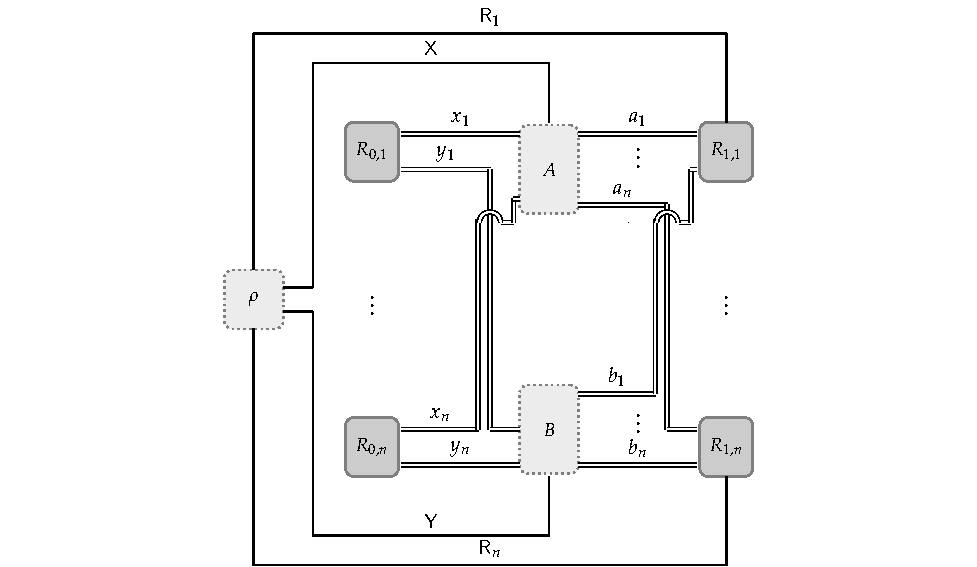
\includegraphics[scale=0.6]{figures/extended_nonlocal_game_parallel_repetition_2.pdf}
	\begin{center}
		\emph{Question:} Do all monogamy-of-entanglement games obey strong parallel repetition? 
	\end{center}
\end{frame}

\begin{frame}
	\frametitle{Parallel repetition of monogamy-of-entanglement games}
	\begin{itemize}
		\item Recall: 
		\begin{align*}
			\omega(G_{\BB84}) = \omega^*(G_{\BB84}) = \cos^2(\pi/8) \approx 0.8536.
		\end{align*}
%		\item For $\abs{\Sigma} = 2$, 
%			\begin{align*}
%				\omega(G) = \omega^*(G).
%			\end{align*}
		\item $G_{\BB84}$ obeys strong parallel repetition\footnote{[Tomamichel, Fehr, Kaniewski, Wehner, (2013)]}:
		\begin{equation*}
			\begin{aligned}
				\omega^*(G_{\BB84}^n) = \omega^*(G_{\BB84})^n = \left( \cos^2(\pi/8) \right)^n.
			\end{aligned}
		\end{equation*}
	\end{itemize}
\end{frame}

\begin{frame}[noframenumbering]
  \vfill
  \centering
  \begin{beamercolorbox}[sep=8pt,center,shadow=true,rounded=true]{title}
    \usebeamerfont{title} Demo Time: Strong parallel repetition of BB84 \\ \textsc{bb84\_parallel\_rep.m}
  \end{beamercolorbox}
  \vfill
  \end{frame}

\begin{frame}
	\frametitle{Upper bounds on strong parallel repetition for monogamy games}
	\begin{theorem}[Tomamichel, Fehr, Kaniewski, Wehner]
		Let $G = (\pi,R)$ be a monogamy game where $\pi$ is uniform over $\Sigma$. It holds that 
		\begin{align*}
			\omega^*(G^n) \leq \left( \frac{1}{\abs{\Sigma}} + \frac{\abs{\Sigma} - 1}{\abs{\Sigma}} \sqrt{c(G)} \right)^n,
		\end{align*}
where $c(G)$ is the ``maximal overlap of measurements'' of the referee
	\begin{align*}
		c(G) = \max_{ \substack{ x,y \in \Sigma \\ x \not= y } } \max_{a,b \in \Gamma} \biggnorm{ \sqrt{R(a|x)} \sqrt{R(b|y)} }^2.
	\end{align*}
	\end{theorem}		
\end{frame}   

\begin{frame}
	\frametitle{Strong parallel repetition for certain monogamy games}
		\begin{theorem}[Johnston, Mittal, R, Watrous]
		Let $G = (\pi,R)$ be a monogamy game where $\abs{\Sigma} = 2$, $\pi$ is uniform over $\Sigma$, and $R(a|x)$ are projective operators. It holds that 
		\begin{align*}
			\omega^*(G^n) = \left( \frac{1}{2} + \frac{1}{2} \sqrt{c(G)} \right)^n. 
		\end{align*}
	\end{theorem}

\end{frame}     

\begin{frame}
	\frametitle{A key proposition and lemma}
	\begin{lemma}
		Let $\Pi_0$ and $\Pi_1$ be nonzero projection operators on $\complex^n$. It holds that 
		\begin{align*}
			\norm{\Pi_0 + \Pi_1} = 1 + \norm{\Pi_0 \Pi_1}.
		\end{align*}
	\end{lemma}
	\vspace{2mm}
	\begin{prop}
		Let $G = (\pi,R)$ be a monogamy-of-entanglement game for which $\Sigma = \{0,1\}$, $\pi$ is uniform over $\Sigma$, and $R(a|x)$ is a projection operator for each $x \in \Sigma$ and $a \in \Gamma$. It holds that 
		\begin{align*}
			\omega(G) = \frac{1}{2} + \frac{1}{2} \max_{a,b \in \Gamma} \biggnorm{R(a|0)R(b|1)}.
		\end{align*}
	\end{prop}
\end{frame}

\begin{frame} 
	\frametitle{Proof of proposition}
	Recall that the unentangled value for any monogamy game $G$ is written as 
	\begin{align*}
		\omega(G) = \max_{f : \Sigma \rightarrow \Gamma} \biggnorm{ \sum_{x \in \Sigma} \pi(x) R(f(x)|x) }.
	\end{align*}			
	\vspace{2mm}
	
	Assuming the lemma stating $\norm{\Pi_0 + \Pi_1} = 1 + \norm{\Pi_0 \Pi_1}$, we have 
	\begin{align*}
		\omega(G) = \max_{a,b \in \Gamma} \biggnorm{ \frac{R(a|0) + R(b|1)}{2} } = \frac{1}{2} + \frac{1}{2} \max_{a,b \in \Gamma} \biggnorm{R(a|0) R(b|1)}.
	\end{align*}
\end{frame}

\begin{frame} 
	\frametitle{Proof of theorem}
	From the proposition that
	\begin{align*}
		\omega(G) = \frac{1}{2} + \frac{1}{2} \sqrt{c(G)}. 
	\end{align*}
	\pause
	Since this is an unentangled strategy, we can assume that Alice and Bob just play every instance optimally (since there is no quantum correlation). It follows then that
	\begin{align*}
		\omega(G^n) = \left( \frac{1}{2} + \frac{1}{2} \sqrt{c(G)} \right)^n. 
	\end{align*}
	\pause
	Recall that the theorem from [Tomamichel, Fehr, Kaniewski, Wehner, (2013)] gives us
	\begin{align*}
		\omega^*(G^n) \leq \left( \frac{1}{2} + \frac{1}{2} \sqrt{c(G)} \right)^n,
	\end{align*}
	which gives us that $\omega^*(G^n) \leq \omega(G^n)$. 
	\pause
	Finally,
	\small{
	\begin{align*}
		\omega^*(G^n) \geq \omega(G^n) \geq \left( \frac{1}{2} + \frac{1}{2} \max_{a,b \in \Gamma} \biggnorm{R(a|0)R(b|1)} \right)^n = \left( \frac{1}{2} + \frac{1}{2} \sqrt{c(G)} \right)^n.
	\end{align*}
	}
\end{frame}

%%%%%%%%%%%%%%%%%%%%%%%%%%%%%%%%%%%%%%%%%%%%%%%%%%%%%
  \section{Open questions}
%%%%%%%%%%%%%%%%%%%%%%%%%%%%%%%%%%%%%%%%%%%%%%%%%%%%%

\begin{frame}
	\frametitle{Unentangled vs.~standard quantum strategies for monogamy-of-entanglement games}	
	\begin{table}
	\centering
	\resizebox{\columnwidth}{!}{%
	\begin{tabular}{|c|c|c|c|c|}
  \hline
    Inputs ($\abs{\Sigma}$) & Outputs ($\abs{\Gamma}$) & $\omega^*(G) = \omega(G)$ & $\omega^*(G^n) = \omega^*(G)^n$ & $\omega_{\ns}(G^n) = \omega_{\ns}(G)^n$  \\
  \hline \hline
  $2$ & $\abs{\Gamma} \geq 1$ & yes & yes\footnotemark & no \\
  \hline
  $3$ & $\abs{\Gamma} \geq 1$ & \textcolor{red}{?} & \textcolor{red}{?} & no \\
  \hline
  $4$ & $3$ & no & ? & no \\
  \hline
\end{tabular}
}
\end{table}
Question: What about $\abs{\Sigma} = 3$?
	\begin{itemize}
			\item Proof technique fails for $\abs{\Sigma} > 2$.
			\item Computational search: 
				\begin{itemize}
					\item Generate random monogamy-of-entanglement games where $\abs{\Sigma} = 3$ and $\abs{\Gamma} \geq 2$. 
					\item $~10^8$ random games generates, no counterexamples found. 
				\end{itemize}
		\end{itemize}

\footnotetext{So long as the measurements used by the referee are projective and the probability distribution, $\pi$, from which the questions are asked is uniform.}
\end{frame}

    
\end{document}